\documentclass[border=5pt]{standalone}
\usepackage{pgfplots}
\usepackage{xcolor}
\pgfplotsset{compat=1.18}

% 自定义样式
\pgfplotsset{
    imp style/.style={red, mark=triangle*, mark size=3pt, line width=0.8pt},
    synflow style/.style={blue, mark=*, mark size=3pt, line width=0.8pt},
    snip style/.style={green!70!black, mark=square*, mark size=3pt, line width=0.8pt},
    baseline style/.style={black, line width=1pt, no marks}
}

\begin{document}
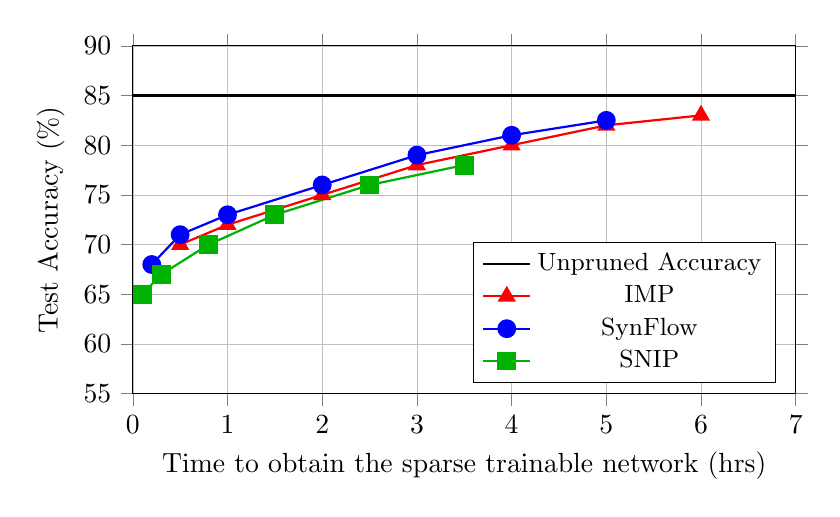
\begin{tikzpicture}
\begin{axis}[
    width=10cm,
    height=6cm,
    xmin=0, xmax=7,
    ymin=55, ymax=90,
    xlabel={Time to obtain the sparse trainable network (hrs)},
    ylabel={Test Accuracy (\%)},
    grid=both,
    grid style={line width=.1pt, draw=gray!10},
    major grid style={line width=.2pt,draw=gray!50},
    legend pos=south east,
    legend style={draw=black, fill=white, font=\small},
    tick align=outside,
    xtick={0,1,2,3,4,5,6,7},
    ytick={55,60,65,70,75,80,85,90},
]

% 未剪枝准确率基线(水平线)
\addplot[baseline style] coordinates {(0,85) (7,85)};
\addlegendentry{Unpruned Accuracy}

% IMP 数据(示例数据点)
\addplot[imp style] coordinates {
    (0.5,70) (1,72) (2,75) (3,78) (4,80) (5,82) (6,83)
};
\addlegendentry{IMP}

% SynFlow 数据(示例数据点)
\addplot[synflow style] coordinates {
    (0.2,68) (0.5,71) (1,73) (2,76) (3,79) (4,81) (5,82.5)
};
\addlegendentry{SynFlow}

% SNIP 数据(示例数据点)
\addplot[snip style] coordinates {
    (0.1,65) (0.3,67) (0.8,70) (1.5,73) (2.5,76) (3.5,78)
};
\addlegendentry{SNIP}

\end{axis}
\end{tikzpicture}
\end{document}